\begin{ccRefFunctionObjectConcept}{Kernel::CompareXAtY_2}
A model for this must provide:

\ccCreationVariable{fo}

\ccMemberFunction{Comparison_result  operator()(const Kernel::Point_2 &p,
                                                const Kernel::Line_2 &h);}
        {compares the $x$-coordinates of $p$ and the horizontal projection
         of \ccStyle{p} on \ccStyle{h}%
         \ccTexHtml{ (Figure~\ref{fig:compare_x_at_y2} (a))}{; see (a) in the
         figure below}.
        }

\begin{ccTexOnly}
\begin{figure}[h]
\centerline{
  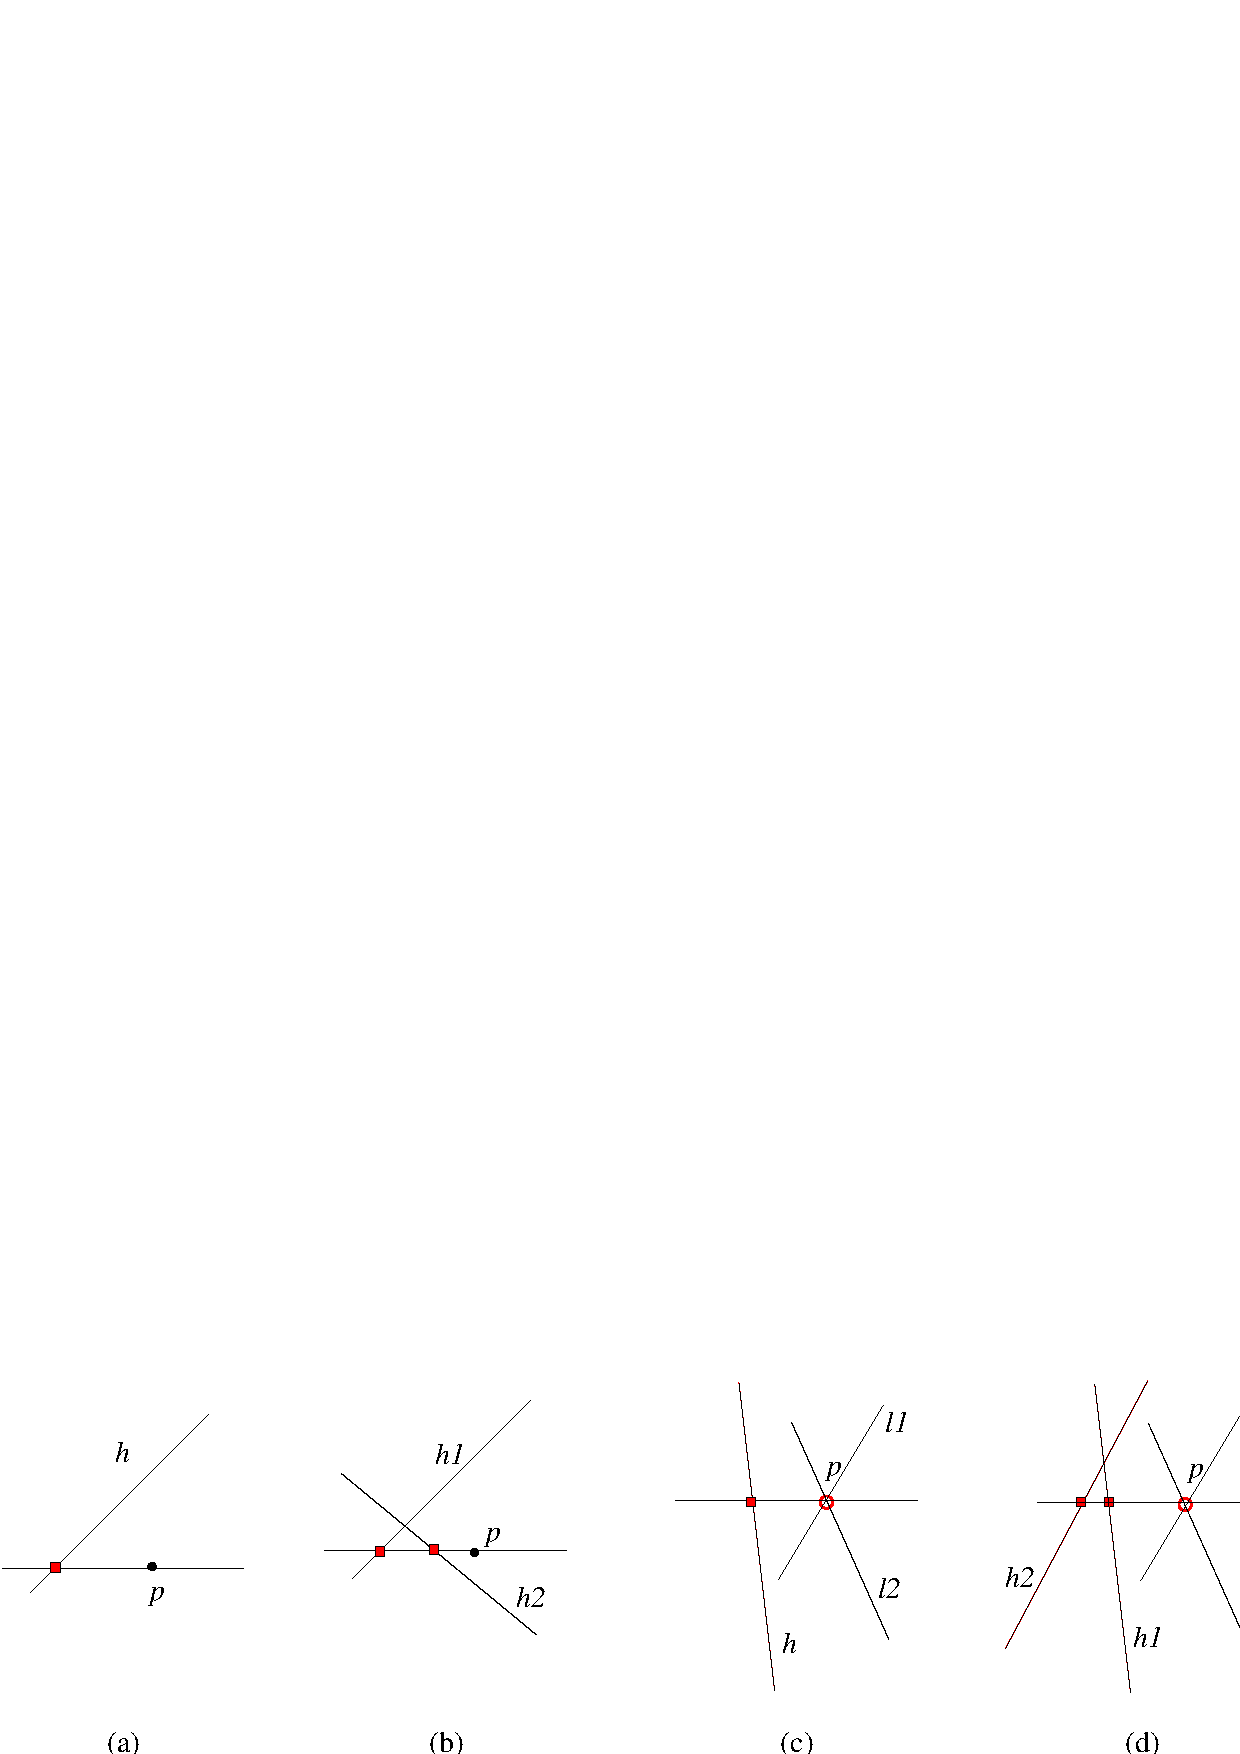
\includegraphics[width=\textwidth]{Kernel_23_ref/fig/compare_x_at_y}}
\caption{Comparison of the $x$-coordinates of the (implicitly given)
         points in the boxes, at a $y$-coordinate. The $y$-coordinate
         is either given explicitly (disc) or implicitly (circle).
         \label{fig:compare_x_at_y2}}
\end{figure}
\end{ccTexOnly}



\ccMemberFunction{Comparison_result operator()(const Kernel::Point_2 &p,
                                               const Kernel::Line_2 &h1,
                                               const Kernel::Line_2 &h2);}
{compares the $x$-coordinates of the horizontal projection 
 of \ccStyle{p} on \ccStyle{h1} and on \ccStyle{h2}%
 \ccTexHtml{ (Figure~\ref{fig:compare_x_at_y2} (b))}{; see (b) in the figure
 below}.
}

\ccMemberFunction{Comparison_result operator()(const Kernel::Line_2 &l1,
                                               const Kernel::Line_2 &l2,
                                               const Kernel::Line_2 &h);}
      {Let $p$ be the \ccHtmlNoLinksFrom{intersection} of lines $l1$ and $l2$.
       This function compares the $x$-coordinates of $p$ and 
       the horizontal projection of \ccStyle{p} on \ccStyle{h}%
       \ccTexHtml{ (Figure~\ref{fig:compare_x_at_y2} (c))}{; see (c) in the
       figure below}.
}



\ccMemberFunction{Comparison_result operator()(const Kernel::Line_2 &l1,
                                               const Kernel::Line_2 &l2,
                                               const Kernel::Line_2 &h1,
                                               const Kernel::Line_2 &h2);}
{Let $p$ be the \ccHtmlNoLinksFrom{intersection} of lines $l1$ and $l2$. This 
 function compares the $x$-coordinates of the horizontal projection of 
 \ccStyle{p} on \ccStyle{h1} and on \ccStyle{h2}%
 \ccTexHtml{ (Figure~\ref{fig:compare_x_at_y2} (d))}{; see (d) in the figure
 below}.
}

\begin{ccHtmlOnly}
<img border=0 src="fig/compare_x_at_y.gif" align=middle 
  alt="Comparison of x at y">
\end{ccHtmlOnly}

\ccRefines
AdaptableFunctor (with three arguments)

\ccSeeAlso
\ccRefIdfierPage{CGAL::compare_x_at_y} \\

\end{ccRefFunctionObjectConcept}
